En esta seccion se detalla el diseño del sistema. Primero haremos una
descripción y justificación de las grandes decisiones arquitéctonicas
tomadas, para luego hacer una descripción más detallada del sistema
entregado.

\subsection{Minilanguage como DSL interna}
Finalmente la DSL se ha implementado por medio de una DSL~interna en
JRuby. Discutiremos las características de las DSL~internas y las
DSL~externas, así como la razón para elegir JRuby.
\subsubsection{DSL internas}
Definición, ventajas, incovenientes, \ldots{}
\subsubsection{DSL externas}
Definición, ventajas, incovenientes, \ldots{}
% JavaCC, ANTLR
\subsubsection{¿Por qué DSL interna?}
\subsubsection{Ruby y JRuby}
\subsubsection{Sintaxis}
\subsubsection{Ejemplos}

\subsubsection{Inyección código malicioso}
Se ha empleado una sandbox, Java Security Architecture, \ldots{}
\subsubsection{Timeouts}
\subsubsection{Manipulación estado intérprete}

\subsection{Servicio sigue estilo arquitectónico REST}
REST\footnote{\emph{Representational state transfer}} es un estilo de
arquitectura software empleado en sistemas distribuidos como la
\emph{World Wide Web}, de ahora en adelante \emph{WWW}.

REST fue desarrollado por Roy Fielding entre otros al mismo tiempo que
se desarrollaba la versión 1.1 del protocolo HTTP. Aun así REST se
puede emplear con otros protocolos si proporcionan mecanismos
adecuados para la transferencia de representación.

El objetivo de la WWW era constituir un espacio común de información
en el que máquinas y usuarios se puedan comunicar.  Los usuarios de
este sistema estarían por todo el mundo, en verias universidades e
institutos de investigación conectados a través de Internet. Las
máquinas así conectadas serían de carácter heterogéneo, haciendo
necesario, con una gran variedad de sistemas operativos y formatos. La
información a distribuir iba desde datos de investigación hasta
listados teléfonicos. El reto era proporcionar un un sistema que
proporcionase una interfaz consistente y universal a todo esta
información estructurada, disponible en el mayor número de plataformas
posibles y capaz de ser aumentada según nuevos usuarios y
organizaciones se uniearan al proyecto.

Como la publicación de información en la WWW era de carácter
voluntario era necesario que las barreras de entrada fueran bajas. Se
eligió \emph{hypermedia} como la interfaz de usuario dada su
simplicidad y generalidad. La misma interfaz puede ser usada
independientemente de la fuente de información. La flexibilidad de los
enlaces permite estructurar sin límites y la manipulación directa de
estos enlaces permite guiar al usuario dentro de la aplicación. Como a
menudo la información dentro de grandes bases de datos es más fácil de
acceder a traves de una búsqueda, WWW también ofrecía la posibilidad
de realizar consultas, respondiendo con hypermedia a los datos
introducidos por el usuario.

Hypermedia distribuida implica que la información pueda estar
almacenada en máquinas remotas. Esto conlleva la transferencia de
grandes cantidades de datos desde el lugar de almacenamiento al lugar
de uso. Para la usabilidad de la hypermedia es básico que la latencia
percibida por parte del usuario sea mímima. Por tanto hay que
minimizar las interacciones con la red.

También es importante que la no disponibilidad de parte del sistema,
no impida a los autores crear contenido de manera local. El lenguaje
de \emph{hypertexto} creado debe de ser sencillo y fácil de crear con
las herramientas existentes.

Otro factor importante es que el protocolo está basado en texto. Esto
facilita la vida de los desarrolladores de aplicaciones, ya que
permite observar y probar el protocolo de una manera directa y
sencilla.

Mientras que la simplicidad facilita la adopción del sistema inicial,
la extensibilidad nos permite mejorar el sistema inicial. Un sistema
con objetivos a largo plazo debe de tener mecanismos para ser
modificado.

Así mismo, el sistema esta orientado a ser desplegado en
Internet. Esto significa que el sistema va a ser usado por diferentes
organizaciones con diferentes objetivos. Normalmente los sistemas de
información son controlados por una única organizacion. Pero en el
caso de la WWW los componentes deben funcionar a pesar de cargas no
anticipadas, datos incorrectos o intencionadamente dañinos, etc. La
escala global conlleva que los clientes no pueden tener conocimiento
de todos los servidores, los servidores no deberían retener estado a
través de varias peticiones. Hypermedia no puede mantener una lista de
páginas que apuntan a un elemento, ya que el número de enlaces puede
ser muy elevado e impredecible.

Dado que la WWW no va a ser controlado por una única organización,
nuevas versiones no se desplegarán homogeneamente. Por tanto,
diferentes versiones de los elementos deben de poder coexistir. Cada
componente debe suponer que nuevas versiones se van a añadir.
Versiones antiguas de un componente deben de ser identificadas de modo
que no interfieran en el funcionamiento de elementos más modernos.

En este contexto, cuando la WWW se empezó a hacer más popular al
principio de los 90 se encontraron numerosas limitaciones a la primera
versión del protocolo HTTP. Las nuevas formas de uso presentaban un
reto para la infraestructura de Internet de aquel momento. Esto
presentaba la necesidad de evolucionar el protocolo HTTP de modo que
fuera mas escalable. ¿Pero que principios usar para guiar su evolución?

La WWW inicial carecía de una arquitectura bien definida. Ante la
existencia de numerosas y a veces contradictorias propuestas para los
diferentes protocolos que forman la WWW, era necesario tener un estilo
arquitectónico. El estilo arquitectónico define una serie de
restricciones; las propuestas han de ser evaluadas contra estas
restricciones buscando posibles conflictos.

Ante esta situación surge el estilo arquitectónico REST con un
especial énfasis en la escalabilidad de la interacción entre
componentes, generalidad de las interfaces, despliegue independiente
de componentes y componentes intermedios para reducir latencia.

REST se define a traves de una serie sucesiva de restricciones que los
elementos de la arquitectura deben seguir. REST es, además, un sistema
híbrido derivado de varios estilos arquitétonicos existentes:

\begin{description}

\item[Cliente-Servidor.] La primera restricción es que el sistema debe
  de ser cliente servidor. La separación de intereses es el principio
  detrás de la separación cliente servidor. Separando los
  requerimientos de la interfaz de usuario de los de almacenamiento de
  datos se mejora la portabilidad de la interfaz de usuario y se
  mejora la escabilidad al simplicar los componentes de servidor. En
  el caso de la WwW, esto permite a los diferentes componentes
  evolucionar independientemente.

\item[Sin Estado.] La comunicación entre un cliente y un servidor debe
  de ser sin estado. Esto significa que cada petición del cliente debe
  contener toda la información necesaria para ser procesada, sin
  beneficiarse de contexto adicional almacenado en el servidor. Por
  tanto estado de la sesión debe de ser almacenado en el cliente.

  Esta restricción induce las propiedades de visibiliad, fiabilidad y
  escalabilidad. La visibilidad es mejorada porque un sistema de
  monitorización no tiene que mirar más alla de una única petición
  para determinar la naturaleza de la petición. La fiabilidad mejora
  porque facilita el proceso de recuperarse de fallos transitorios. La
  escalabilidad mejora porque no tener que almancenar estado entre
  peticiones, permite al servidor liberar recursos de manera rápida y
  simplifica la implementación.

  La desventaja de un protocolo sin estado es que el rendimiento de la
  red puede reducirse al tener que transmitir más datos repetidos, ya
  que no se puede mantener en el servidor un contexto
  compartido. Aparte dejar el estado en el cliente, reduce el control
  del servidor sobre el comportamiento consistente de la aplicación,
  ya que la aplicación depende de la implementación correcta del
  comportamiento por los clientes a lo largo de diferentes versiones.

\item[Caché.] Para mejorar la eficiencia de la red, se añaden
  restricciones de caché. Se requiere que los datos dentro de una
  respuesta sean marcados como cacheables o no cacheables. Si una
  respuesta es cacheable, se permite que la caché de un cliente
  reutilice esa respuesta para peticiones posteriores.

  La ventaja fundamental de una caché es que permite eliminar completa
  o parcialmente algunas interacciones, aumentando la eficiencia, la
  escalabilidad y el rendimiento percibido por el usuario al reducir
  la latencia. El inconveniente es que una caché puede reducir la
  fiabilidad, si los datos obtenido de la caché difieren
  considerablemente de los que se obtendrían en una nueva petición.

  Las restricciones presentadas hasta ahora son las que definieron el
  estado inicial de la arquitectura de la WWW.

\item[Interfaz Uniforme.] Esta es la característica principal que
  distingue REST de otros estilos arquitecturales. Al aplicar el
  principio de la generalidad a la interfaz del componente, la
  arquitectura global es simplificada y la visibilidad de las
  interacciones es mejorada. Los servicios ofrecidos están
  desacoplados de las implementaciones, lo que facilita la evolución
  independiente de los mismos. El inconveniente es que una interfaz
  uniforme reduce la eficiencia, ya que la información es transmitida
  en un formato estandarizado en vez de uno específico para la
  aplicación. La interfaz uniforme definida por REST esta diseñada
  para ser eficiente en el caso de transferencias de Hypermedia de
  grano grueso, el caso más tipico en la WWW.

  Cuando un enlace es seleccionado, la información necesita ser
  llevada desde el lugar de almacenamiento hasta la localización donde
  va a ser usado. Esto es a diferencia de otros paradigmas
  distribuidos, en los que es muchas más veces más sencillo llevar el
  agente procesador a los datos. Para poder llevar a cabo esta
  transferencia, se transfiere una \emph{representación} del recurso
  en un formato correspondiente a algún tipo estándar. El formato se
  selecciona dinámicamente basado en las características y los deseos
  del cliente y la naturaleza del recurso. Si la representación es el
  mismo formato que el recurso o es derivada de la original, permanece
  oculto tras la interfaz. El formato de la represeentación es
  conocido como tipo MIME\cite{MIME}. Una representación puede ser
  incluida y procesada por el destinatario en acorde a los datos de
  control del mensaje y la naturaleza del tipo de datos.

  En REST otra abstracción clave a la hora de ofrecer una interfaz
  uniforme son los recursos. Cualquier información que se puede
  nombrar puede ser un recurso: una imagen, un documento, un servicio,
  una colección de recursos, un objeto físico, etc. Cualquier concepto
  que pueda ser referido mediante un enlace de hypertexto es un
  recurso. Un recurso es un conjunto de entidades que en un momento
  dado son equivalentes entre si. Estas entidades son representaciones
  del recurso. Algunos recursos son estáticos, una vez creados no
  varían. Otros son altamente variables y a lo largo del tiempo pasan
  a tener representaciones diferentes. Esta definición abstracta de un
  recurso, permite abarcar numerosas fuentes de información empleando
  la misma interfaz basada en recursos. En la WWW los recursos son
  referenciados por medio de las URI\footnote{\emph{Uniform Resource
      Identifiers}}, combinación de las URL\footnote{\emph{Uniform
      Resource Locator}} y las URN\footnote{\emph{Uniform Resource
      Names}}.

  Podemos ver que cada servidor en la WWW ofrece una interfaz
  abstracta para acceder a los recursos y transferirlos. Cada recurso
  puede ser manipulado con una serie de verbos predefinidos: GET,
  POST, PUT y DELETE. Por lo tanto un servicio REST define un espacio
  de nombres por medio de recursos que pueden ser operados por medio
  de una interfaz genérica basada en los verbos HTTP más tipos
  estándar MIME. Esta serie de recursos definidos por un servicio han
  de tener una semántica clara. La idea es que los nombres de los
  recursos permanezcan más o menos fijos, mientras que las
  representaciones pueden variar.

\item[Sistema en Capas.] Esta restricción mejora el comportamiento para
  requisitos de escalabilidad a nivel de Internet. Esta restricción
  permite a una arquitectura estar compuesta por capas jerárquicas de
  modo que cada capa solo pueda ver más alla de la capa con la que
  están interaccionando. Limitando la visibilidad a la capa inmediata,
  reducimos la complejidad global y promovemos independencia con
  respecto a las otras capas. Las capas se pueden usar para encapsular
  servicios desfasados y para proteger nuevos servicios de clientes
  desfasados, simplificando los componentes al mover funcionalidad
  raramente usada a un intermediario. Los intermediarios también
  pueden ser usados para aumentar la escalabilidad al permitir el uso
  de reparto de carga de un servicio a través de múltiples redes y
  nodos.

\item[Código bajo Demanda.] REST permite que la funcionalidad de los
  clientes pueda ser extendida, descargando y ejecutando código en
  forma de applets y scripts. Esto simplifica los clientes al reducir
  el número de características que tienen que estar
  preinstaladas. Permitir nuevas características a posteriori mejora
  la extensibilidad del sistema.
\end{description}

Una vez hemos descrito REST veamos que nos aporta en relación a DARE y
porque se ha decidido escogerlo.

Consideramos que REST es más práctico. No conlleva la carga conceptual
de, por ejemplo SOAP\cite{SOAP}. Como la WWW está basada en los
conceptos de REST, todos los programadores están familiarizados con
ellos. Mientras es cierto que el soporte de SOAP es extenso y suelen
existir herramientas para facilitar su uso, en muchas plataformas no
es una opción. Por ejemplo, si queremos crear una aplicación web que
acceda al servicio, como es el caso de una de las posibles
ampliaciones de este proyecto. Ver~\ref{MASHUP_REF} en
pág.~\pageref{MASHUP_REF}.

Además REST nos facilita proporcionar diferentes representaciones de
los recursos definidos. Por ejemplo, nos ha facilitado proporcionar
las respuestas tanto en XML como en JSON. Esto es SOAP habría de
realizarse de manera completamente manual.

El hecho de que REST nos obligue a ofrecer un servicio sin estado,
facilita la escalabilidad del mismo en gran manera. Nos permite
introducir un balanceador de carga o proxy inverso. El balanceador de
carga repartirá las peticiones recibidas entre todos los nodos
disponibles. Si se añade un nodo, éste es capaz de empezar a atender
peticiones inmediatamente, ya que no hay un contexto asociado a las
peticiones anteriores. Además nos ayuda a mantener un servicio
altamente fiable. Si uno de los nodos falla, la petición se puede
enviar a cualquiera de los otros nodos, permitiendo que el servicio
siga funcionando. No hacen falta por tanto, complicados mecanismos de
\emph{failover}.

Al usar REST podemos emplear el soporte del protocolo HTTP para
cachear resultados. Esto nos permite evitar transferencias
innecesarias, ahorrando ancho de banda y reduciendo la
latencia. Consideramos que está es una de las claves para obtener un
alto rendimiento en situaciones en las que varios Robots están siendo
accedidos continuamente.

Así mismo, consideramos que una API REST es más fácil de evolucionar y
menos frágil que una equivalente en SOAP. HTTP incorpora mecanismos
para negociar las respuestas dadas, facilitando la coexistencia de
diversas versiones de clientes. En SOAP los nuevos clientes tendrían
que utilizar métodos con nombres distintos o habría que desfasar las
versiones antiguas de los clientes inmediatamente.


\subsubsection{JAX-RS\cite{JAXRS}}

Como hemos explicado la WWW se basa en REST como estilo
arquitectónico. Sería perfectamente viable implementar el servicio
utilizando algún framework o tecnología web típica: CGI, PHP,
Servlets, Struts, Ruby on Rails, etc. Aun así, la mayoría de los
frameworks no fomentan el seguimiento de los principios REST de una
manera rigurosa.

Al final hemos decidido usar el framework JAX-RS. No se trata de una
librería en concreto, sino de una especificación. Ha sido diseñada con
el propósito de crear aplicaciones web siguiendo los principios
REST. El objetivo de la especificación es crear una API de alto nivel,
con un estilo declarativo usando anotaciones.

Hemos considerado que su funcionamiento era adecuado para nuestras
necesidades. Para las necesidades de este proyecto se muestra como una
buena opción. Además tiene una parte de cliente lo que facilitaría la
creación de la librería para la parte Java.

Existen varias implementaciones de esta API. Nos hemos decantado por
la implementación por defecto, Jersey\cite{JERSEY}.

\subsection{MongoDB como Sistema Almacenamiento}
\subsubsection{Opciones valoradas}
\subsubsection{MongoDB}
\subsubsection{Razón elección}

\subsection{Arquitectura Backend}
\subsubsection{Embarrassingly parallel}
http://en.wikipedia.org/wiki/Embarrassingly\_parallel
\subsubsection{Descripción Arquitectura}
\subsubsection{Mover partes aplicación a otros nodos}

\subsection{Clojure como lenguaje de programación}
Características, razón elección, \ldots{}
\subsubsection{Librerías Empleadas}
\begin{description}
\item{CongoMongo} es \ldots{}
\item{Lamina} es\ldots{}
\item{Aleph} es\ldots{}
\item{Gloss} es\ldots{}
\end{description}

\subsection{DARE como procesos sin estado}
http://www.12factor.net/port-binding
http://www.12factor.net/processes
Hablar de por qué se eligió Jetty en vez de Glassfish. Por qué modo
embebido.

\subsection{Librería para Python}
\subsubsection{httplib2}
% rest.py a fondo?
\subsection{Interfaz Línea Comandos en Python}

\subsection{Componentes}
A continuación veamos una visión general del proyecto desde el punto
de vista de un diagrama de componentes UML. En el se muestran los
componentes presentes y las relaciones entre los mismos. A mayores
vamos a realizar una breve descripción de cada uno de ellos:

\begin{description}

\item[minilenguaje:] Es el componente que implementa la DSL definida
  por el proyecto. Este lenguaje se ha denominado minilenguaje. Es
  responsable de transformar la DSL en el formato XML entendido por
  \emph{aAUTOMATOR Runtime}\footnote{Está contenido dentro del
    artefacto \emph{StringEditor}}. Está implmentado en JRuby y
  Java. La parte en JRuby se encarga de definir una DSL interna y la
  parte Java ofrece una API a la misma.
\item[DARE-domain:] Define un modelo de dominio del sistema. Facilita
  una comprensión conceptual del sistema, abstrayéndonos de otras
  consideraciones. Contiene clases como Robot, ExecutionResult y
  PeriodicalExecution. Instancias de estas clases son creadas cuando
  se obtienen datos del sistema de almacenamiento. Está implementado
  en Java.
\item[DARE-war:] Es una aplicación web Java. Contiene todos los
  componentes dentro del recuadro servicio. Puede ser desplegado en
  cualquier servidor de aplicaciones JEE y/o contenedor de servlets.

  Siguiendo el patrón MVC\footnote{Modelo Vista Controlador} este
  modelo es el responsable de la parte de vista y controlador. Utiliza
  la api JAX-RS para lleva a cabo esta labor. Utiliza a DARE-domain
  como modelo y DARE-backend ofrecería servicios de persistencia y
  ejecución.

  Este componente ha sido concebido de modo que se puede desplegar en
  varios nodos, ya que se sigue una filosofía
  \emph{share-nothing}. Para ellos nos hacemos valer de las
  características sin estado de REST. Es decir, podemos tener varios
  servidores web ejecutándose en distintos nodos. Está implementado en
  Java.

\item[DARE-backend:] Es el componente encargado de comunicarse con la
  base de datos MongoDB tanto para leer como para escribir los objetos
  definidos en DARE-domain. Recibe también las peticiones de ejecución
  para aAUTOMATOR. Luego utilizando la parte cliente de DARE-workers
  las reparte entre los procesos \emph{worker} que se están
  ejecutando.

\item[DARE-workers:] Este componente está compuesto por una parte
  cliente que lanza peticiones de ejecución a aAUTOMATOR. La parte
  servidor, de ahora en adelante \emph{worker}, interpreta esas
  peticiones y hace el trabajo correspondiente. Uno o varios de estos
  workers pueden estar lanzados en función de las necesidades de
  escalabilidad y fiabilidad necesarios.

  Cada worker es un proceso por lo que alguno de ellos podría dejar de
  funcionar y DARE podría seguir ofreciendo su servicio. Además al ser
  cada uno un proceso se pueden ejecutar localmente en el mismo nodo o
  repartirlo a traves de varios nodos del cluster. La parte cliente es
  capaz de descubrirlos y repartir la carga de peticiones entre los
  workers. Aparte comprueba continuamente el estado de salud de los
  workers para que el servicio continúe funcionando aun en la
  presencia de errores en los workers.

 Tanto la parte servidor como cliente están implementados en Clojure.

\item[DARE-util:] Es un cajón de sastre donde se encuentran diversas
  funciones de utilidad usadas por varios otros módulos.

\item[DARE-web:] Este módulo se utiliza para facilitar el despliegue
  de la aplicación. Toma el fichero \emph{war} con la aplicación y lo
  ejecuta creando un servicio web. Para ello emplea el contenedor de
  servlets embebido, Jetty\cite{JETTY}. Jetty es un contenedor de
  servlets ligero, por lo que es especialmente adecuado para lanzar
  numerosas instancias de la aplicación. Este componente está
  implementado en Clojure.

\item[DARE-java:] %TODO extract
\item[DARE-python:] Este módulo implemente la librería cliente para
  Python, así como la aplicación de línea de comandos. Como se ha
  descrito anteriormente usa httplib2 para llevar a cabo la
  comunicación con el servicio.

  La aplicación de línea de comandos está contenida en este componente
  y utiliza la librería creada para llevar a cabo su
  funcionalidad. Como es lógico está implementado en Python.
\end{description}

\begin{landscape}
\begin{figure}[p]
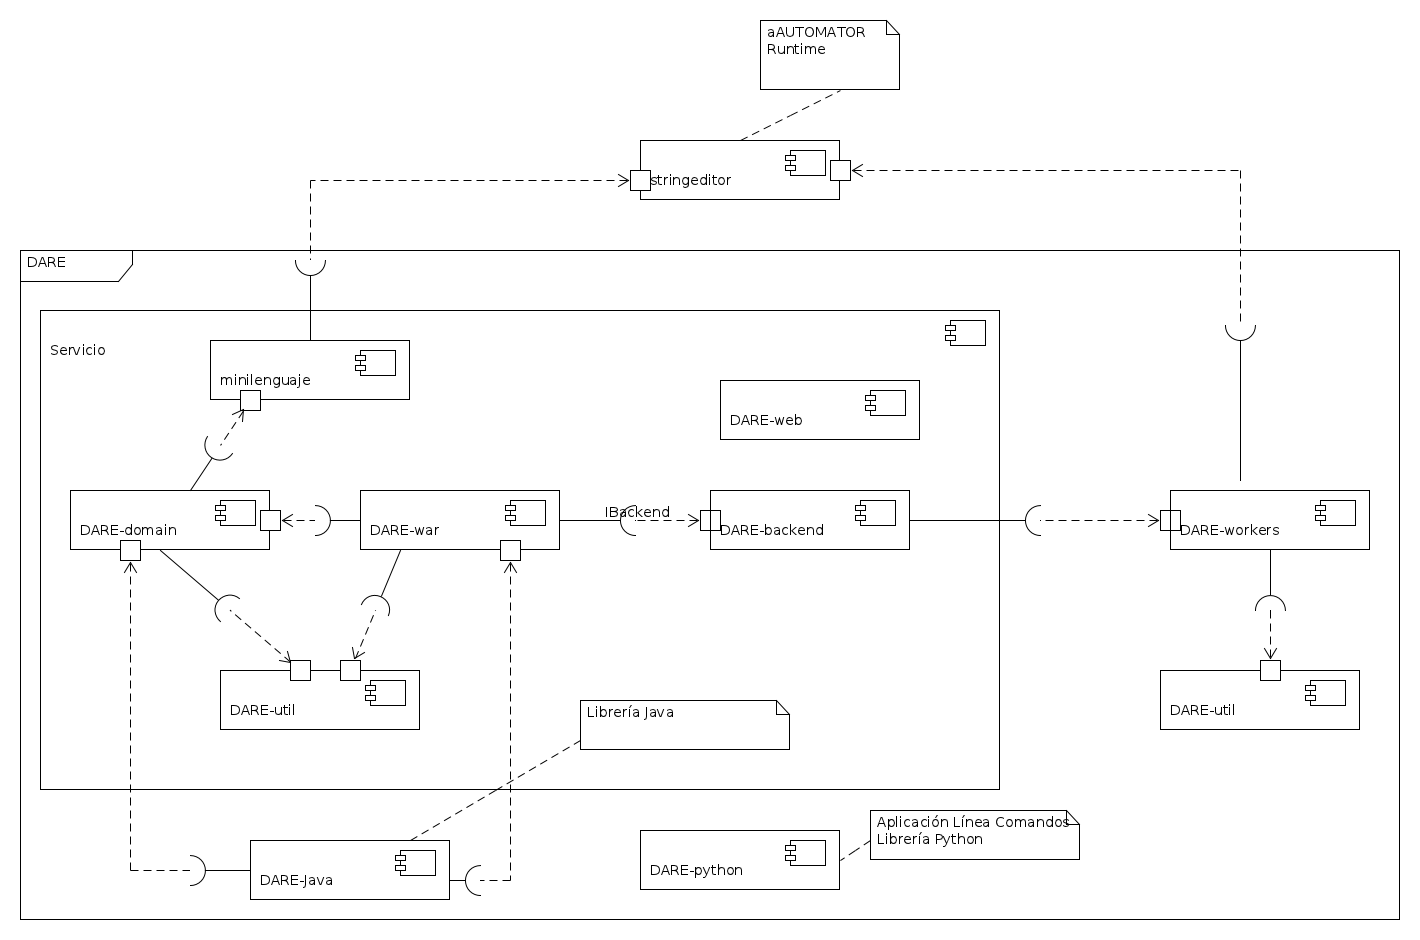
\includegraphics[width=1.4\textwidth]{chapters/technical-manual/diagrams/diagrama_componentes.png}
\caption{Diagrama Componentes DARE}\label{diagrama_componentes_dare}
\end{figure}
\end{landscape}


\subsubsection{Diagrama clases minilenguaje}

\subsubsection{Descripción Implementación transformer.rb}
Descripción general \ldots{}
% transformer.rb en modo literario

\subsubsection{Diagrama clases DARE-war}
\begin{figure}[!hbp]
\makebox[\textwidth]{\framebox[5cm]{\rule{0pt}{5cm}}}
\caption{Diagrama dominio}
\end{figure}

\subsubsection{Diagrama clases DARE-backend}
% a fondo backend/core.clj?
\subsubsection{Diagrama clases DARE-workers}
% a fondo workers/client.clj, workers/server.clj?

\subsubsection{Esquema datos Sistema Almacenamiento}
